\section{Examples of the Previously Mentioned Places (26K,27P)}

% -- Chart 26.1 ---------------------------------------------
\subsection*{\textit{[Chart 15 Fortunate, A Leader]}}
\addcontentsline{toc}{subsection}{\textit{[Chart 15 [GH L188] Fortunate, A Leader]}}

Let the \Sun, \Moon, \Jupiter, \Mercury\xspace be in \Leo, \Saturn, Ascendant in \Libra, \Mars\xspace in \Gemini \footnote{GH places \Mars\xspace in \Aquarius.}, \Venus\xspace in \Cancer
\footnote{\textit{Greek Horoscopes} dates the chart (L188) to approximately August 10, 188 AD (p.130)}.

\clearpage
\begin{wrapfigure}[15]{R}{7cm}
\centering
%\vspace{-20pt}
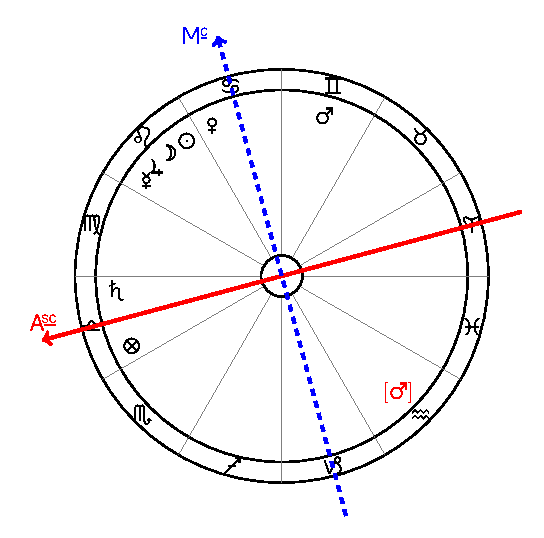
\includegraphics[width=0.68\textwidth]{charts/2_26_1}
\caption{Chart 15 [II.26.1, GH L188]}
\label{fig:chart15}
\end{wrapfigure}

This person was fortunate, a leader, dictatorial, possessed of royal fortune, and in solid possession of great property. 

The Lot of Fortune, Daimon, and Basis were located in the same sign <\Libra>, and \Venus, the ruler of these Lots, was at MC in \Cancer. 

The ruler <\Jupiter> of the triangle <\Leo-\Aries-\Sagittarius> and the ruler <\Mercury> of the Exaltation <\Gemini> were found in <the XI Place of> Good Daimon and in Accomplishment.

\newpage
% -- Chart 26.2 ----------------------------------------------
\subsection*{\textit{[Chart 16 A Governor]}}
\addcontentsline{toc}{subsection}{\textit{[Chart 16 [GH L86] A Governor]}}

Another example: \Sun, \Mercury, \Venus, Ascendant in \Leo, \Saturn\xspace in \Taurus, \Jupiter\xspace in \Sagittarius, \Mars\xspace in \Libra, \Moon\xspace in \Capricorn
\footnote{\textit{Greek Horoscopes} dates the chart (L86) to approximately August 11, 86 AD (p.94).}

\clearpage
\begin{wrapfigure}[8]{R}{7cm}
\centering
\vspace{-20pt}
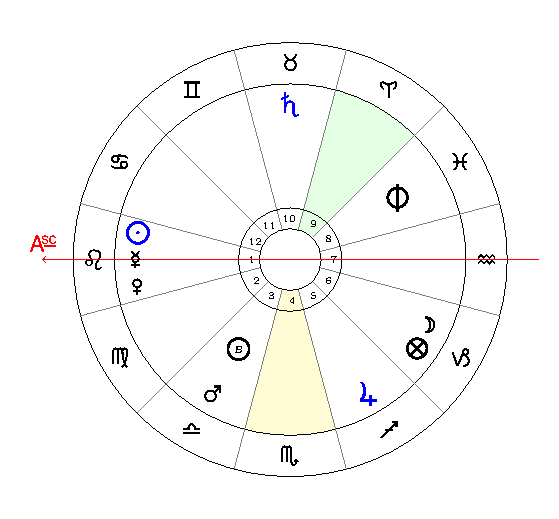
\includegraphics[width=0.68\textwidth]{charts/2_26_2}
\caption{Chart 16 [II.26.2, GH L86]}
\vspace{-150pt}
\label{fig:chart16}
\end{wrapfigure}

This person was a governor, a master of life and death because the stars were found in their own domains
\footnote{The chart is diurnal, triplicity rulers are \Sun-\Jupiter-\Saturn. Only the \Sun\xspace in \Leo\xspace and \Jupiter\xspace in \Sagittarius\xspace are in their own ``domains'' (domiciles). \Saturn\, has no essential dignity in \Taurus; he could possibly be in his own bounds. \textsl{Greek Horoscopes} puts him around 9° \Taurus\, which is in \Saturn's bounds, according to Valens (see Book III Table 3.1 The Order of the Terms) but are \Mercury's bounds according to the Egyptians.}.

\newpage

% -- Chart 26.3 ----------------------------------------------
\subsection*{\textit{[Chart 17 Exile and Violent Death ]}}
\addcontentsline{toc}{subsection}{\textit{[Chart 17 [GH L78] Exile and Violent Death]}}

Another example: \Sun, \Moon, \Jupiter, Ascendant in \Aries, \Saturn, \Venus in \Aquarius, \Mars\xspace in \Gemini, \Mercury\xspace in \Pisces
\footnote{\textit{Greek Horoscopes} dates the chart (L78) to approximately April 1, 78 AD (p.91).}

\clearpage
\begin{wrapfigure}[14]{R}{7cm}
\centering
\vspace{-20pt}
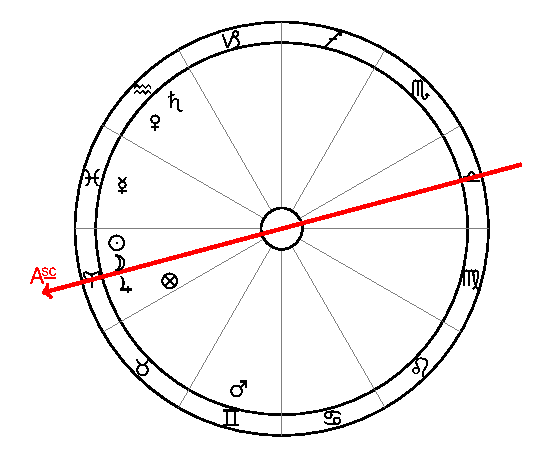
\includegraphics[width=0.68\textwidth]{charts/2_26_3}
\caption{Chart 17 [II.26.3, GH L78]}
\label{fig:chart17}
\end{wrapfigure}

This person was commanding and dictatorial because the rulers <\Sun, \Jupiter> of the triangle <\Leo-\Sagittarius-\Aries> were found to be at an angle and in the Ascendant. 

The Lot of Fortune, Daimon, and Basis, as well as the Exaltation, were located in the same place <\Aries>. The ruler of these, \Mars, being unfavorably situated and not in aspect with the <III> Place\footnote{This doesn't make much sense. No planet is in aspect to the ``place'' (house) it occupies and \Mars\xspace is sextile the 1st House, the place it rules. GH says there's a lacuna in the Kroll text leaving the original meaning in doubt. It's possible the original meaning meant the placement and aspect were not fortunate as \Mars\xspace is opposite the chart (day) sect being a night planet, and in decline. So a sextile, usually fotunate, being a half-trine, is instead, unfortunate, it has ``opposite effects''.} had the opposite effects,
\textbf{/94K/} both exile and violent death; for it was the ruler of the new moon <in \Aries>.

\newpage
% -- Chart 26.4 ----------------------------------------------
\subsection*{\textit{[Chart 18 Fame, Wealth, Exile and Suicide ]}}
\addcontentsline{toc}{subsection}{\textit{[Chart 18 [GH L101] Exile and Suicide]}}

Another example: \Sun, \Jupiter, \Venus\xspace in \Pisces, \Moon\xspace in \Libra, \Mars\xspace in \Cancer, \Mercury\xspace in \Aquarius, \Saturn\xspace in \Scorpio, Ascendant in \Leo
\footnote{\textit{Greek Horoscopes} dates the chart (L101) to approximately March 5, 101 AD (p.99).}.

\clearpage
\begin{wrapfigure}[14]{R}{7cm}
\centering
\vspace{-20pt}
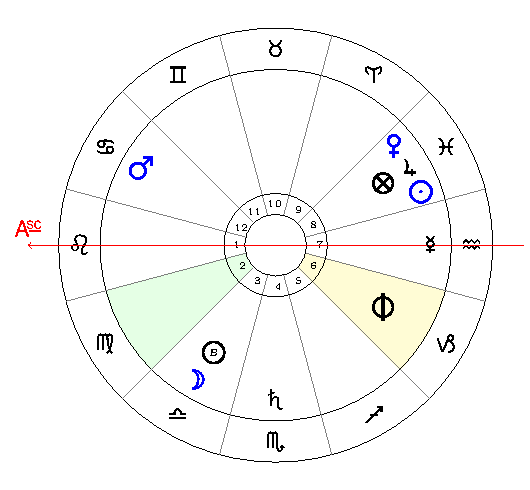
\includegraphics[width=0.68\textwidth]{charts/2_26_4}
\caption{Chart 18 [II.26.4, GH L101,III]}
\label{fig:chart18}
\end{wrapfigure}


This person was famous and wealthy because the \Sun\xspace was attended by benefics and was found situated in the Lot of Fortune <\Pisces> with its houseruler <\Jupiter>. But since \textbf{/90P/} the co-rulers of the same sect <\Mars, \Moon> of the triangle <\Pisces-\Cancer-\Scorpio> were
unfavorably situated, and the ruler <\Saturn> of Daimon <\Capricorn> was turned away\footnote{\Saturn\xspace \Semisextile\xspace \Moon? The \Semisextile\xspace (30\deg) and the \Quincunx\xspace (150\deg) aspects are often described as ``turned away.''}, this person was exiled and committed suicide. In addition \Mars\xspace was in opposition to Accomplishment <\Capricorn>, and the ruler <\Mercury> of the Exaltation <\Virgo> did not have a suitable place, but was afflicted by \Saturn, which was in superior [\Square] aspect.

Therefore \mndl as I have already said, if most of the configurations or their rulers are found in suitable places,
the native will be famous and spectacular in his living. If some <configurations and rulers> are favorably
situated, others unfavorably, rank and fortune will be transitory.

\newpage